\documentclass[]{article}
\usepackage{lmodern}
\usepackage{amssymb,amsmath}
\usepackage{ifxetex,ifluatex}
\usepackage{fixltx2e} % provides \textsubscript
\ifnum 0\ifxetex 1\fi\ifluatex 1\fi=0 % if pdftex
  \usepackage[T1]{fontenc}
  \usepackage[utf8]{inputenc}
\else % if luatex or xelatex
  \ifxetex
    \usepackage{mathspec}
  \else
    \usepackage{fontspec}
  \fi
  \defaultfontfeatures{Ligatures=TeX,Scale=MatchLowercase}
\fi
% use upquote if available, for straight quotes in verbatim environments
\IfFileExists{upquote.sty}{\usepackage{upquote}}{}
% use microtype if available
\IfFileExists{microtype.sty}{%
\usepackage{microtype}
\UseMicrotypeSet[protrusion]{basicmath} % disable protrusion for tt fonts
}{}
\usepackage[margin=1in]{geometry}
\usepackage{hyperref}
\hypersetup{unicode=true,
            pdftitle={Introduction to visualising spatial data in R},
            pdfauthor={Prof.~Uttam Kumar, Mayur Rajwani},
            pdfborder={0 0 0},
            breaklinks=true}
\urlstyle{same}  % don't use monospace font for urls
\usepackage{color}
\usepackage{fancyvrb}
\newcommand{\VerbBar}{|}
\newcommand{\VERB}{\Verb[commandchars=\\\{\}]}
\DefineVerbatimEnvironment{Highlighting}{Verbatim}{commandchars=\\\{\}}
% Add ',fontsize=\small' for more characters per line
\newenvironment{Shaded}{}{}
\newcommand{\AlertTok}[1]{\textcolor[rgb]{1.00,0.00,0.00}{\textbf{#1}}}
\newcommand{\AnnotationTok}[1]{\textcolor[rgb]{0.38,0.63,0.69}{\textbf{\textit{#1}}}}
\newcommand{\AttributeTok}[1]{\textcolor[rgb]{0.49,0.56,0.16}{#1}}
\newcommand{\BaseNTok}[1]{\textcolor[rgb]{0.25,0.63,0.44}{#1}}
\newcommand{\BuiltInTok}[1]{#1}
\newcommand{\CharTok}[1]{\textcolor[rgb]{0.25,0.44,0.63}{#1}}
\newcommand{\CommentTok}[1]{\textcolor[rgb]{0.38,0.63,0.69}{\textit{#1}}}
\newcommand{\CommentVarTok}[1]{\textcolor[rgb]{0.38,0.63,0.69}{\textbf{\textit{#1}}}}
\newcommand{\ConstantTok}[1]{\textcolor[rgb]{0.53,0.00,0.00}{#1}}
\newcommand{\ControlFlowTok}[1]{\textcolor[rgb]{0.00,0.44,0.13}{\textbf{#1}}}
\newcommand{\DataTypeTok}[1]{\textcolor[rgb]{0.56,0.13,0.00}{#1}}
\newcommand{\DecValTok}[1]{\textcolor[rgb]{0.25,0.63,0.44}{#1}}
\newcommand{\DocumentationTok}[1]{\textcolor[rgb]{0.73,0.13,0.13}{\textit{#1}}}
\newcommand{\ErrorTok}[1]{\textcolor[rgb]{1.00,0.00,0.00}{\textbf{#1}}}
\newcommand{\ExtensionTok}[1]{#1}
\newcommand{\FloatTok}[1]{\textcolor[rgb]{0.25,0.63,0.44}{#1}}
\newcommand{\FunctionTok}[1]{\textcolor[rgb]{0.02,0.16,0.49}{#1}}
\newcommand{\ImportTok}[1]{#1}
\newcommand{\InformationTok}[1]{\textcolor[rgb]{0.38,0.63,0.69}{\textbf{\textit{#1}}}}
\newcommand{\KeywordTok}[1]{\textcolor[rgb]{0.00,0.44,0.13}{\textbf{#1}}}
\newcommand{\NormalTok}[1]{#1}
\newcommand{\OperatorTok}[1]{\textcolor[rgb]{0.40,0.40,0.40}{#1}}
\newcommand{\OtherTok}[1]{\textcolor[rgb]{0.00,0.44,0.13}{#1}}
\newcommand{\PreprocessorTok}[1]{\textcolor[rgb]{0.74,0.48,0.00}{#1}}
\newcommand{\RegionMarkerTok}[1]{#1}
\newcommand{\SpecialCharTok}[1]{\textcolor[rgb]{0.25,0.44,0.63}{#1}}
\newcommand{\SpecialStringTok}[1]{\textcolor[rgb]{0.73,0.40,0.53}{#1}}
\newcommand{\StringTok}[1]{\textcolor[rgb]{0.25,0.44,0.63}{#1}}
\newcommand{\VariableTok}[1]{\textcolor[rgb]{0.10,0.09,0.49}{#1}}
\newcommand{\VerbatimStringTok}[1]{\textcolor[rgb]{0.25,0.44,0.63}{#1}}
\newcommand{\WarningTok}[1]{\textcolor[rgb]{0.38,0.63,0.69}{\textbf{\textit{#1}}}}
\usepackage{graphicx,grffile}
\makeatletter
\def\maxwidth{\ifdim\Gin@nat@width>\linewidth\linewidth\else\Gin@nat@width\fi}
\def\maxheight{\ifdim\Gin@nat@height>\textheight\textheight\else\Gin@nat@height\fi}
\makeatother
% Scale images if necessary, so that they will not overflow the page
% margins by default, and it is still possible to overwrite the defaults
% using explicit options in \includegraphics[width, height, ...]{}
\setkeys{Gin}{width=\maxwidth,height=\maxheight,keepaspectratio}
\IfFileExists{parskip.sty}{%
\usepackage{parskip}
}{% else
\setlength{\parindent}{0pt}
\setlength{\parskip}{6pt plus 2pt minus 1pt}
}
\setlength{\emergencystretch}{3em}  % prevent overfull lines
\providecommand{\tightlist}{%
  \setlength{\itemsep}{0pt}\setlength{\parskip}{0pt}}
\setcounter{secnumdepth}{0}
% Redefines (sub)paragraphs to behave more like sections
\ifx\paragraph\undefined\else
\let\oldparagraph\paragraph
\renewcommand{\paragraph}[1]{\oldparagraph{#1}\mbox{}}
\fi
\ifx\subparagraph\undefined\else
\let\oldsubparagraph\subparagraph
\renewcommand{\subparagraph}[1]{\oldsubparagraph{#1}\mbox{}}
\fi

%%% Use protect on footnotes to avoid problems with footnotes in titles
\let\rmarkdownfootnote\footnote%
\def\footnote{\protect\rmarkdownfootnote}

%%% Change title format to be more compact
\usepackage{titling}

% Create subtitle command for use in maketitle
\providecommand{\subtitle}[1]{
  \posttitle{
    \begin{center}\large#1\end{center}
    }
}

\setlength{\droptitle}{-2em}

  \title{Introduction to visualising spatial data in R}
    \pretitle{\vspace{\droptitle}\centering\huge}
  \posttitle{\par}
    \author{Prof.~Uttam Kumar, Mayur Rajwani}
    \preauthor{\centering\large\emph}
  \postauthor{\par}
      \predate{\centering\large\emph}
  \postdate{\par}
    \date{2019-12-25. See
\href{https://github.com/rajwanimayur/SpatialAnalysis}{github.com/rajwanimayur/SpatialAnalysis.pdf}
for latest version}


\begin{document}
\maketitle

{
\setcounter{tocdepth}{2}
\tableofcontents
}
\hypertarget{preface}{%
\section{Preface}\label{preface}}

The objective of this tutorial is to provide its readers the necessary
skills to visualise diverse range of geographical and non-geographical
datasets and make meaningful inferences.

The tutorial is practical in nature, where you will load-in, visualise
and manipulate spatial data. The tutorial requires basic knowledge of R,
thus if you do not have prior experience of using R, it is advised to
follow the tutorial -
\href{https://cran.r-project.org/doc/contrib/Paradis-rdebuts_en.pdf}{\emph{R
for beginners by Emmanuel Paradis}}.

\hypertarget{why-r}{%
\subsection{Why R?}\label{why-r}}

\begin{enumerate}
\def\labelenumi{\arabic{enumi}.}
\tightlist
\item
  R is free and open-source.
\item
  Using R, researchers can reproduce their work and verify other
  people's work.
\item
  R has numerous packages available for spatial data analysis,
  statistical modelling, econometrics, visualising and more.
\end{enumerate}

Now you know the usage and benefits of using R for spatial data
analysis, its now time to delve deeper into it. To that end, this
tutorial is organised as follows:

\begin{enumerate}
\def\labelenumi{\arabic{enumi}.}
\tightlist
\item
  \textbf{Introduction} : provides a guide to R's syntax and preparing
  you for the tutorial.
\item
  \textbf{Handling Spatial Data in R}: describing basic spatial
  functions in R
\item
  \textbf{Data Preparation} : which include creating and manipulating
  spatial data for visualisations.
\item
  \textbf{Data Visualisation - Making Interactive Maps in R} : this
  section will demonstrate map making with R's advanced visualisation
  tools, namely \textbf{ggmap}.
\item
  \textbf{Analysing Spatial Data} : In this section, we analyse the road
  accidents data for all states in India, over all the period of four
  years altogether.
\end{enumerate}

To distinguish between prose and code, please be aware of the following
typographic conventions used in this document: R code
(e.g.~\texttt{plot(x,\ y)}) is written in a \texttt{monospace} font and
package names (e.g.~\textbf{rgdal}) are written in \textbf{bold}. A
double hash (\texttt{\#\#}) at the start of a line of code indicates
that this is output from R. Lengthy outputs have been omitted from the
document to save space, so do not be alarmed if R produces additional
messages: you can always look up them up on-line.

\begin{quote}
As an advice, we encourage you to play with the code. Try out new
things, explore different ways to do similar tasks and enjoy the
learning ride.
\end{quote}

This tutorial makes use of RStudio, an IDE(Integrated Development
Environment) with code editor and tools for debugging and visualization.
RStudio makes it easier to use R. To download Rstudio, visit -
\url{https://www.rstudio.com}

\clearpage

\hypertarget{introduction}{%
\section{1. Introduction}\label{introduction}}

R has a huge and growing number of spatial data packages. We recommend
taking a quick browse on R's main website to see the spatial packages
available at: \url{http://cran.r-project.org/web/views/Spatial.html}. We
highlight few packages below, which are used extensively in this
tutorial. One is advised to download all recommended packages
beforehand.

\begin{itemize}
\tightlist
\item
  \textbf{sp} : This package provides classes and methods for spatial
  data; utility functions for plotting maps, working with coordinates,
  etc.
\item
  \textbf{ggplot2} : The most popular package for data visualization.
\item
  \textbf{ggmap} : extends the plotting package ggplot2 for maps. ggmap
  provides functions to visualise spatial data on top of static maps
  from sources like Google Maps, Open Street Maps, cloudmade and stamen.
\item
  \textbf{rgdal} : This package provides methods for working with
  importing and exporting different raster and vector geospatial data
  formats; Coordinate Reference Systems; projections, etc.
\item
  \textbf{rgeos} : R's interface to the powerful vector processing
  library geos. It provides functions for handling operations on
  topologies.
\item
  \textbf{dplyr} and \textbf{tidyr} : fast and concise data manipulation
  packages
\item
  \textbf{broom} : Takes messy output of built-in functions in R, and
  turns them into tidy data frames.
\end{itemize}

Some packages may already be installed on your computer. To test if a
package is installed, try to load it using the \texttt{library}
function; for example, to test if \textbf{ggplot2} is installed, type
\texttt{library(ggplot2)} into the console window. If there is no output
from R, this is good news: it means that the library has already been
installed on your computer.

If you get an error message,you will need to install the package using
\texttt{install.packages("ggplot2")}. The package will download from the
Comprehensive R Archive Network (CRAN); if you are prompted to select a
`mirror', select one that is close to current location. If you have not
done so already, install these packages on your computer now. A
\href{http://stackoverflow.com/questions/8175912/load-multiple-packages-at-once}{quick
way} to do this in one go is to enter the following lines of code:

\begin{Shaded}
\begin{Highlighting}[]
\NormalTok{x <-}\StringTok{ }\KeywordTok{c}\NormalTok{(}\StringTok{"sp"}\NormalTok{, }\StringTok{"ggplot2"}\NormalTok{, }\StringTok{"ggmap"}\NormalTok{, }\StringTok{"rgdal"}\NormalTok{, }\StringTok{"rgeos"}\NormalTok{, }\StringTok{"dplyr"}\NormalTok{, }\StringTok{"tidyr"}\NormalTok{, }\StringTok{"broom"}\NormalTok{, }\StringTok{"ggsn"}\NormalTok{) }
\CommentTok{# install.packages(x) # warning: uncommenting this may take a number of minutes}
\KeywordTok{lapply}\NormalTok{(x, library, }\DataTypeTok{character.only =} \OtherTok{TRUE}\NormalTok{) }\CommentTok{# load the required packages}
\end{Highlighting}
\end{Shaded}

\hypertarget{handling-spatial-data-in-r}{%
\section{2. Handling Spatial Data in
R}\label{handling-spatial-data-in-r}}

In this section, we will look at mapping and geographical data handling
capabilities of R. The aim of this section is to develop basic building
blocks for the Spatial data analysis in later sections.

All code and data used for this tutorial can be downloaded from
\href{https://github.com/rajwanimayur/SpatialAnalysisInR}{github
repository}. Click on the ``Download ZIP'' button on the right hand side
of the screen and once downloaded, unzip this to a new folder on your
computer.

Open the existing ``GISTutorial'' project using File -\textgreater{}
Open File\ldots{} on the top menu. Alternatively, you can also use the
project menu to open the project or create a new one. It is recommended
to use RStudio's projects to organise R work and organise files into
sub-folders and avoid digital clutter.

The first file we are going to load into R Studio is the ``states''
shapefile located in the \texttt{Data/States} folder of the project. It
is worth looking at this input dataset in your file browser before
opening it in R. You will notice that there are several files named
``states'', all with different file extensions. This is because a
shapefile is actually made up of a number of different files, such as
.prj, .dbf and .shp. You could also try opening the file ``states.shp''
file in a conventional GIS such as QGIS to see what a shapefile contains.
You should also open ``states.dbf'' in a spreadsheet program such as
Microsoft Excel, or LibreOffice Calc. to see what this file contains.
Once you think you understand the input data, it's time to open it in R.
There are a number of ways to do this, the most commonly used and
versatile of which is \textbf{readOGR}. This function, from the
\textbf{rgdal} package, automatically extracts the information regarding
the data.

\textbf{rgdal} is R's interface to the ``Geospatial Abstraction Library
(GDAL)'' which is used by other open source GIS packages such as QGIS
and enables R to handle a broader range of spatial data formats.

\begin{Shaded}
\begin{Highlighting}[]
\KeywordTok{library}\NormalTok{(rgdal)}
\NormalTok{states_raw <-}\StringTok{ }\KeywordTok{readOGR}\NormalTok{(}\DataTypeTok{dsn =} \StringTok{"Data/States/states.shp"}\NormalTok{, }\DataTypeTok{stringsAsFactors =} \OtherTok{FALSE}\NormalTok{)}
\NormalTok{states <-}\StringTok{ }\NormalTok{states_raw}
\end{Highlighting}
\end{Shaded}

In the second line of code above the \textbf{readOGR} function is used
to load a shapefile and assign it to a new spatial object called
\emph{states}.

\textbf{readOGR} is a \emph{function} of the `\textbf{rgdal} package,
the first \emph{argument} of which \textbf{dsn:} ``data source name'',
the file or directory of the geographic data to be loaded. Recent
developments of \textbf{rgdal} package doesn't require specification of
layer file any longer. \emph{states} is now an spatial data object with
boundary data specifying the state name.

\hypertarget{the-structure-of-spatial-data-in-r}{%
\subsection{The Structure of spatial data in
R}\label{the-structure-of-spatial-data-in-r}}

Spatial objects like the \textbf{states} object are made up of a number
of different \emph{slots}. \emph{slots} provides the object oriented
representation of data in R. Each slot in an object (here \emph{states})
is a component of the object; like components (that is, elements) of a
list, this may be extracted and set, using the function `slot()' or more
often the operator `\,``@''\,'. However, they differ from list
components in important ways. First, slots can only be referred to, by
name and not by position, and there is no partial matching of names as
with list elements.

Lets have a look at slots in \textbf{states} object.

\begin{Shaded}
\begin{Highlighting}[]
\KeywordTok{slotNames}\NormalTok{(states)}
\end{Highlighting}
\end{Shaded}

\begin{verbatim}
## [1] "data"        "polygons"    "plotOrder"   "bbox"        "proj4string"
\end{verbatim}

In the above slots, the \textbf{data} slot and \textbf{polygons} are of
interest to us. The \emph{data} slot contains non geographic attribute
data (in this case the state name), while \emph{polygons} slot (or
\emph{lines} slot for line data) contains geographic information of
latitude and longitude. Thus the data slot is considered as the
attribute table and the geometry slot is the polygons that make up the
physical boundaries.

\hypertarget{basic-plotting}{%
\subsection{Basic Plotting}\label{basic-plotting}}

Now we have seen structure of our spatial object states, we will now
look at plotting them.

\begin{Shaded}
\begin{Highlighting}[]
\KeywordTok{plot}\NormalTok{(states) }\CommentTok{# Not shown, will plot the shapefile}
\end{Highlighting}
\end{Shaded}

\emph{plot} is one of the most useful functions in R. It can be used to
draw maps for spatial data objects as well as conventional graphs. This
is often referred as polymorphism.

R also provide powerful subsetting capabilities that can be accessed
very concisely using square brackets.

\begin{Shaded}
\begin{Highlighting}[]
\CommentTok{#We first see the classes of all variables in spatial dataset}
\KeywordTok{sapply}\NormalTok{(states}\OperatorTok{@}\NormalTok{data, class)}
\end{Highlighting}
\end{Shaded}

\begin{verbatim}
##       ST_NM 
## "character"
\end{verbatim}

As evident, \texttt{ST\_NM} is of type character, Thus we do not need
any form of type conversion. Next we select states whose name starts
with ``A'' only.

\begin{Shaded}
\begin{Highlighting}[]
\NormalTok{states}\OperatorTok{@}\NormalTok{data[}\KeywordTok{startsWith}\NormalTok{(states}\OperatorTok{$}\NormalTok{ST_NM, }\StringTok{"A"}\NormalTok{),]}
\end{Highlighting}
\end{Shaded}

\begin{verbatim}
## [1] "Andaman & Nicobar Island" "Arunanchal Pradesh"      
## [3] "Assam"                    "Andhra Pradesh"
\end{verbatim}

Next we will plot these selected states.

\begin{Shaded}
\begin{Highlighting}[]
\NormalTok{sel <-}\StringTok{ }\KeywordTok{startsWith}\NormalTok{(states}\OperatorTok{$}\NormalTok{ST_NM, }\StringTok{"A"}\NormalTok{)}
\KeywordTok{plot}\NormalTok{(states[sel,])  }\CommentTok{# See Figure 1}
\end{Highlighting}
\end{Shaded}

\begin{figure}
\centering
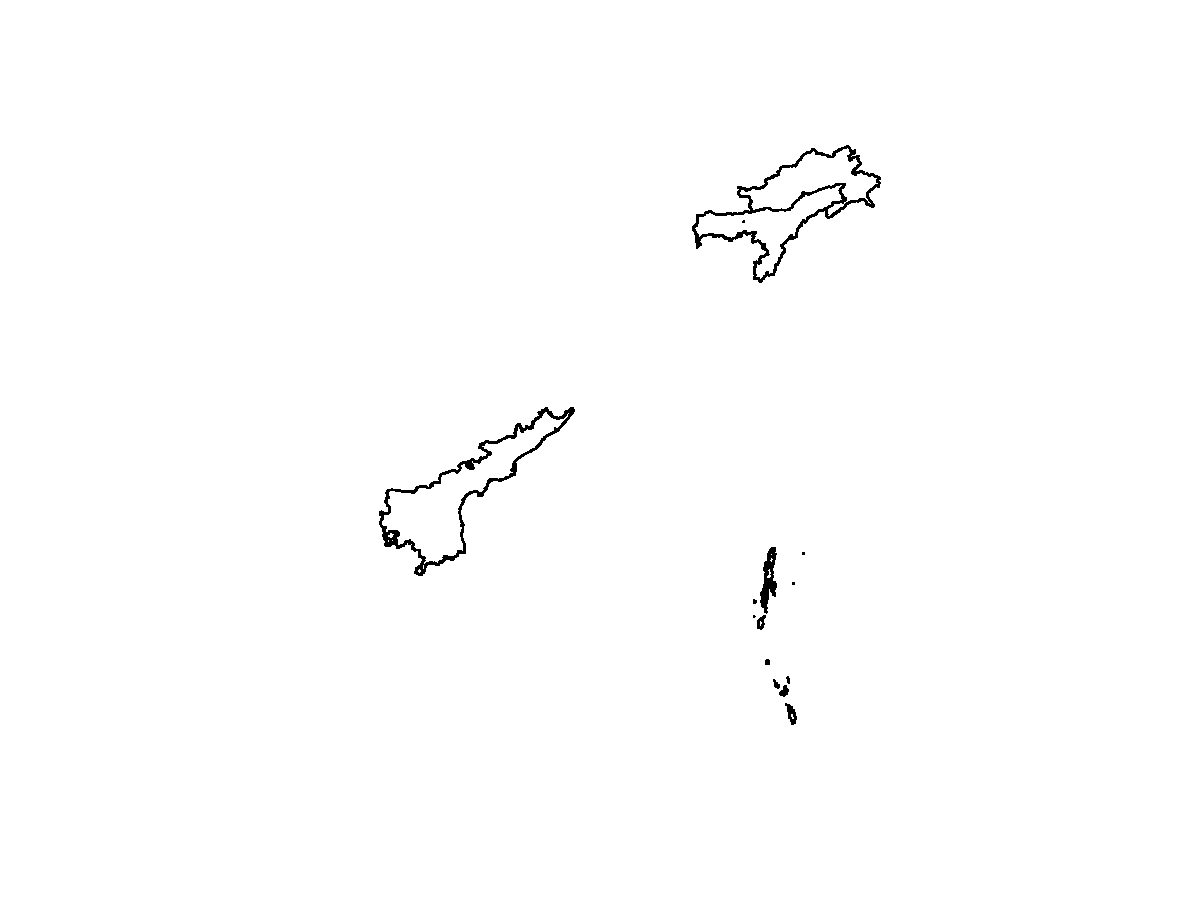
\includegraphics{TutorialNotebook_files/figure-latex/unnamed-chunk-8-1.pdf}
\caption{States whose names starts with A}
\end{figure}

The plot is quite useful, but it only display the areas we selected. In
order to see the areas that meets the selection criteria, in context
with the other areas of the map we simply use the \emph{add = TRUE}
argument after the initial plot.

\begin{Shaded}
\begin{Highlighting}[]
\CommentTok{#Plotting initial graph}
\KeywordTok{plot}\NormalTok{(states, }\DataTypeTok{col =} \StringTok{"lightgray"}\NormalTok{)}
\NormalTok{sel <-}\StringTok{ }\KeywordTok{startsWith}\NormalTok{(states}\OperatorTok{$}\NormalTok{ST_NM, }\StringTok{"A"}\NormalTok{)}
\KeywordTok{plot}\NormalTok{(states[sel,], }\DataTypeTok{col =} \StringTok{"blue"}\NormalTok{, }\DataTypeTok{add =} \OtherTok{TRUE}\NormalTok{)  }\CommentTok{#See Figure 2}
\end{Highlighting}
\end{Shaded}

\begin{figure}
\centering
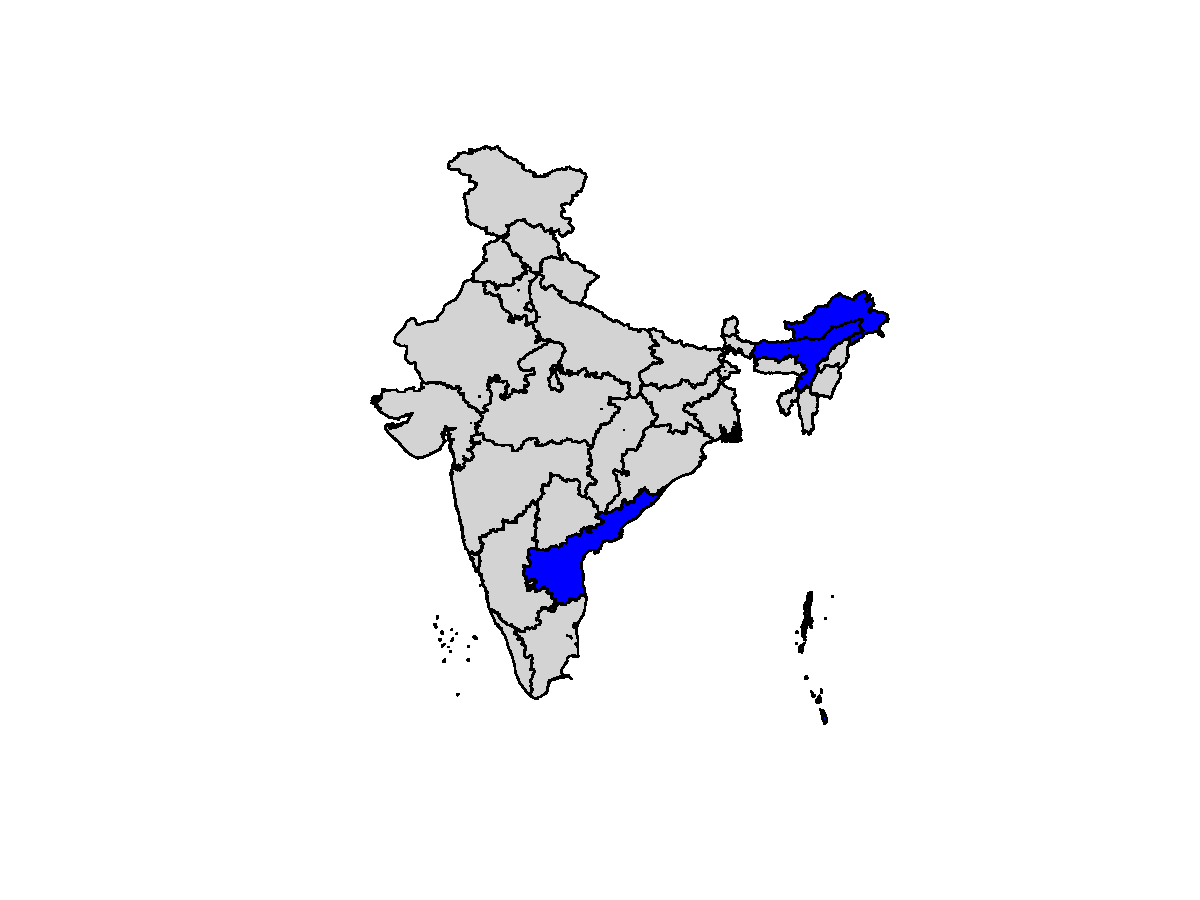
\includegraphics{TutorialNotebook_files/figure-latex/unnamed-chunk-9-1.pdf}
\caption{Map of India, highlighting the states whose name starts with
`A'}
\end{figure}

\hypertarget{projections-setting-and-transforming-crs-in-r}{%
\subsection{Projections: setting and transforming CRS in
R}\label{projections-setting-and-transforming-crs-in-r}}

The next section requires the spatial object to have planar projections.
Thus, we first modify our spatial object to have a planar projection and
then carry our further exploration of data.

\begin{Shaded}
\begin{Highlighting}[]
\NormalTok{states}\OperatorTok{@}\NormalTok{proj4string}
\end{Highlighting}
\end{Shaded}

\begin{verbatim}
## CRS arguments:
##  +proj=longlat +datum=WGS84 +no_defs +ellps=WGS84 +towgs84=0,0,0
\end{verbatim}

The \emph{Coordinate Reference System} (CRS) of spatial objects defines
where they are placed on the Earth's surface. The above R code displays
the summary of `\texttt{proj4string}' slot of \texttt{states}. The
information that follows represents its CRS. Spatial data should always
have a CRS. If no CRS information is provided, and the correct CRS is
known, it can be set as follow:

\begin{Shaded}
\begin{Highlighting}[]
\CommentTok{# Remove the existing CRS Information first.}
\KeywordTok{proj4string}\NormalTok{(states) <-}\StringTok{ }\OtherTok{NA_character_}
\KeywordTok{proj4string}\NormalTok{(states) <-}\StringTok{ }\KeywordTok{CRS}\NormalTok{(}\StringTok{"+init=epsg:27700"}\NormalTok{)}
\end{Highlighting}
\end{Shaded}

R issues a warning when the CRS is changed. This is so the user knows
that they are simply changing the CRS, not \emph{reprojecting} the data.
An easy way to refer to different projections is via
\href{http://www.epsg-registry.org/}{EPSG codes}.We used CRS system
\texttt{27700} representing the British National Grid. Also its worth
mentioning the commonly used CRS worldwide is `WGS84' with EPSG code
\texttt{epsg:4326}.

Now we have projected spatial object, we will now select and plot only
zones that are close to centroid of India.
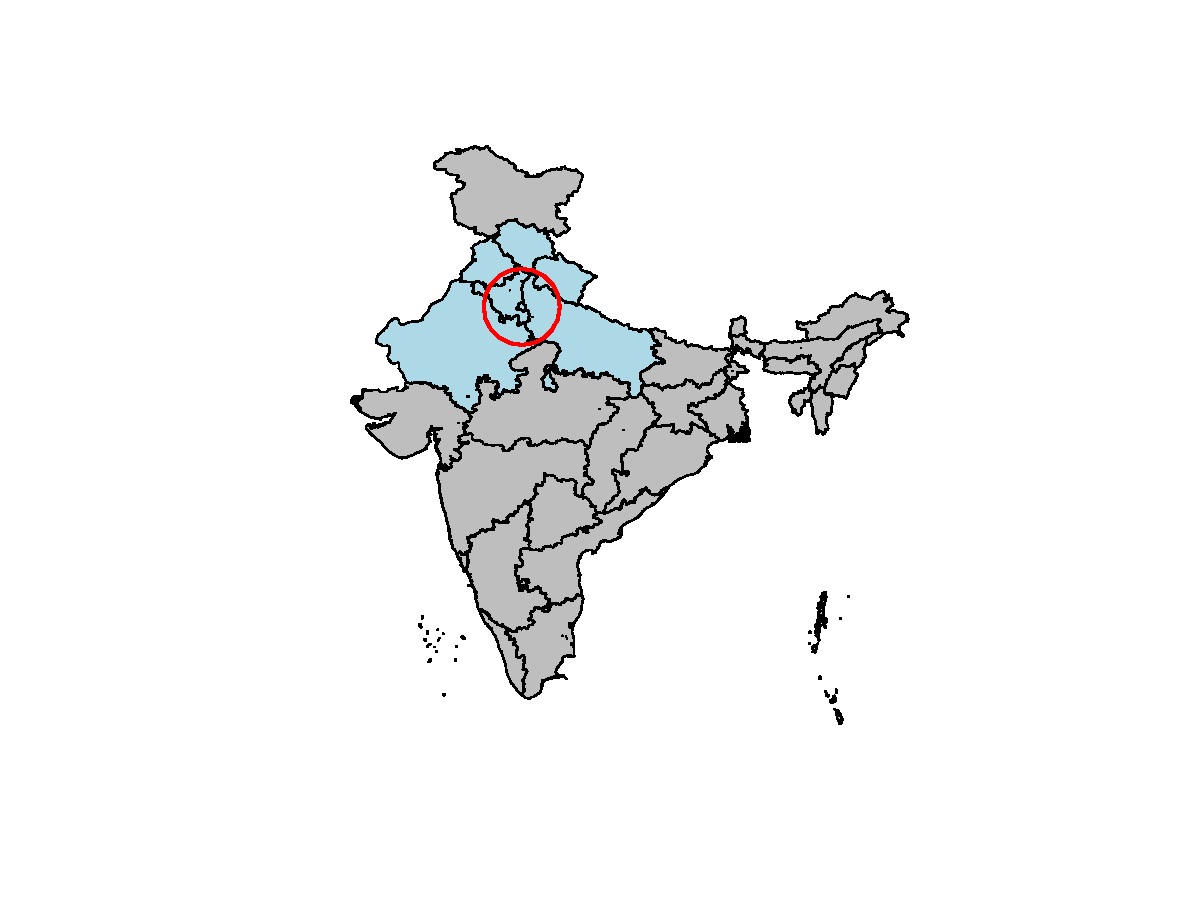
\includegraphics{TutorialNotebook_files/figure-latex/unnamed-chunk-12-1.pdf}

\hypertarget{data-preparation}{%
\section{3. Data Preparation}\label{data-preparation}}

In the following section we shall use the dataset representing road
accidents in India \href{https://data.gov.in/node/6619609}{Source -
https://data.gov.in/node/6619609}. The data provides statewise accidents
record over the year 2014 to 2017. The available data is a non-spatial
data, i.e, it doesn't contain location information of latitude and
longitude. The Spatial data we have, contains only names of state as an
attribute. It does not contain any useful information. How can we add
more infomration to our existing spatial objects? The following section
will answer this. Before we delve into the details, we will re-load our
``states'' spatial object from ``states\_raw''

\begin{Shaded}
\begin{Highlighting}[]
\NormalTok{states <-}\StringTok{ }\NormalTok{states_raw}
\end{Highlighting}
\end{Shaded}

The non-spatial object we are going to join our \texttt{states} object
contains States/UTs road accidents records. The file contains comma
seperated values and can be opened using any spreadsheet program like MS
Excel.

\begin{Shaded}
\begin{Highlighting}[]
\CommentTok{# Read csv file and Create a new data frame object accidents}
\NormalTok{accidents_raw<-}\StringTok{ }\KeywordTok{read.csv}\NormalTok{(}\StringTok{"Data/Road_Accidents_2017-Annuxure_Tables_4.csv"}\NormalTok{, }\DataTypeTok{stringsAsFactors =} \OtherTok{FALSE}\NormalTok{)}
\NormalTok{accidents <-}\StringTok{ }\NormalTok{accidents_raw }\CommentTok{#Avoid Re-Reading of CSV File}
\end{Highlighting}
\end{Shaded}

Note that accidents is a Data Frame containing 36 rows and 19 variables.
We can also infer that column \emph{States.UTs} is of type \texttt{chr},
i.e a String(Hence, no need for type coercion), and rest other columns
are \texttt{integer} and \texttt{double}. Before we join the two
datasets, we check for consistency among the joining variable. Since the
state names should ubiquitous, we check for values in
\texttt{accidents\$States.UTS} which do not occur in
\texttt{states\$ST\_NM} and vice - versa. We need to handle these
missing values accordingly.

\begin{Shaded}
\begin{Highlighting}[]
\NormalTok{accidents}\OperatorTok{$}\NormalTok{States.UTs[}\OperatorTok{!}\NormalTok{accidents}\OperatorTok{$}\NormalTok{States.UTs }\OperatorTok\StringTok{ }\NormalTok{states}\OperatorTok{$}\NormalTok{ST_NM]}
\end{Highlighting}
\end{Shaded}

\begin{verbatim}
## [1] "Arunachal Pradesh"         "Andaman & Nicobar Islands"
## [3] "Dadra & Nagar Haveli"      "Delhi"
\end{verbatim}

\begin{Shaded}
\begin{Highlighting}[]
\NormalTok{states}\OperatorTok{$}\NormalTok{ST_NM[}\OperatorTok{!}\NormalTok{states}\OperatorTok{$}\NormalTok{ST_NM }\OperatorTok\StringTok{ }\NormalTok{accidents}\OperatorTok{$}\NormalTok{States.UTs]}
\end{Highlighting}
\end{Shaded}

\begin{verbatim}
## [1] "Andaman & Nicobar Island" "Arunanchal Pradesh"      
## [3] "Dadara & Nagar Havelli"   "NCT of Delhi"
\end{verbatim}

We have found the discrpenacies as a typrographical error. Therefore we
edit the states name in \texttt{states\$ST\_NM} from R's data editor.
The following line of code will open an editor, you need to correct the
errors manually. \textbf{Note} - Do not change the order of values.

\begin{Shaded}
\begin{Highlighting}[]
\NormalTok{states}\OperatorTok{@}\NormalTok{data <-}\StringTok{ }\KeywordTok{edit}\NormalTok{(states}\OperatorTok{@}\NormalTok{data)}
\end{Highlighting}
\end{Shaded}

Now, we can join our data. We make use of package \textbf{dplyr} to join
two data frames. One can also use the \texttt{merge} function for the
same.

\begin{Shaded}
\begin{Highlighting}[]
\KeywordTok{library}\NormalTok{(dplyr)  }\CommentTok{#load dplyr}
\NormalTok{states}\OperatorTok{@}\NormalTok{data <-}\StringTok{ }\KeywordTok{inner_join}\NormalTok{(states}\OperatorTok{@}\NormalTok{data, accidents, }\DataTypeTok{by =} \KeywordTok{c}\NormalTok{(}\StringTok{'ST_NM'}\NormalTok{ =}\StringTok{ 'States.UTs'}\NormalTok{))}
\end{Highlighting}
\end{Shaded}

The \texttt{*join} command assume, by default, that matching variables
have same name. Here we specify the association between two data frames,
using the `\texttt{by}' argument.

\clearpage

\hypertarget{making-interactive-maps-in-r-using-ggmap}{%
\section{4. Making Interactive Maps in R, using
ggmap}\label{making-interactive-maps-in-r-using-ggmap}}

\hypertarget{ggplot2}{%
\subsection{ggplot2}\label{ggplot2}}

In this section we create slightly different plots in R, using
\textbf{ggplot2} package. The pacakage is implentation of the Grammar of
Graphics (Wilkinson 2015) - a general scheme for data visualisation that
breaks up graphs into semantic components such as scales, layers and
facets. It makes plotting of complex plots easier by providing a
programmatic interface for variable specification, displaying of plots
and other general visual properties. Thus \textbf{ggplot2} requires
minimal changes if there is an underlying data change or we decide to
change from bar plot to scatter plot.

\textbf{ggplot2} is a
\href{http://docs.ggplot2.org/current/}{well-documented} package and
contains number of default options that match good visualisation
practices.

We now begin exploring \textbf{ggplot2} with a scatter plot for
attribute data in \texttt{states} object. We first set up the data we
need to plot. For this, we first subset the data to few columns. Here we
select variables that specify the ``Total Number of Persons Injured'' in
a calendar year. Next we rename those columns to represent only year
number, since our dataset now represent only single feature, namely
``Total Number of Persons Injured''

\begin{Shaded}
\begin{Highlighting}[]
\CommentTok{#Create a temporary dataframe for analysis purpose}
\NormalTok{df <-}\StringTok{ }\NormalTok{states}\OperatorTok{@}\NormalTok{data[,}\DecValTok{1}\OperatorTok{:}\DecValTok{5}\NormalTok{]}
\CommentTok{#Rename Columns to Year only}
\KeywordTok{colnames}\NormalTok{(df) <-}\StringTok{ }\KeywordTok{gsub}\NormalTok{(}\StringTok{"}\CharTok{\textbackslash{}\textbackslash{}}\StringTok{D+}\CharTok{\textbackslash{}\textbackslash{}}\StringTok{.}\CharTok{\textbackslash{}\textbackslash{}}\StringTok{.}\CharTok{\textbackslash{}\textbackslash{}}\StringTok{."}\NormalTok{, }\StringTok{""}\NormalTok{, }\KeywordTok{colnames}\NormalTok{(df))}
\end{Highlighting}
\end{Shaded}

Next we \texttt{tidy} the data and
\texttt{\textquotesingle{}gather\textquotesingle{}}(from \textbf{tidyr}
package) columns values into rows. This creates a single variable called
\textbf{Year}, values of which are stored in another variable
\textbf{Persons\_Injured}. This allows us to create a single tuple of
form \textless ST\_NM, Year, Person\_Injured\textgreater{} representing
all the information contained in our dataset. It makes visualization of
our data easy.

\begin{Shaded}
\begin{Highlighting}[]
\KeywordTok{library}\NormalTok{(tidyr)}
\NormalTok{df.m <-}\StringTok{ }\KeywordTok{gather}\NormalTok{(df, }\DataTypeTok{key =} \StringTok{"Year"}\NormalTok{, }\DataTypeTok{value =} \StringTok{"Persons_Injured"}\NormalTok{, }\KeywordTok{colnames}\NormalTok{(df)[}\DecValTok{2}\OperatorTok{:}\DecValTok{5}\NormalTok{])}
\end{Highlighting}
\end{Shaded}

We will require this dataframe in latter section, hence We save our
\texttt{df.m} object for latter use.

\begin{Shaded}
\begin{Highlighting}[]
\KeywordTok{saveRDS}\NormalTok{(}\DataTypeTok{object =}\NormalTok{ df.m, }\DataTypeTok{file =} \StringTok{"Data/Statewise_Yearly_Road_Accidents_India.Rds"}\NormalTok{)}
\end{Highlighting}
\end{Shaded}

Now we are ready for setting up our \texttt{ggplot} object. The
\texttt{ggplot} object takes \texttt{df.m} ( a dataframe object) as
input. We then specify the type of plot we want, in our case we draw a
scatter plot (using \texttt{geom\_point()} function). We also define the
aesthetics, i.e, variables of graph. Here we call variables \emph{Year}
and \emph{Persons\_Injured} as variables \emph{x} and \emph{y} of our
graph. Next we plot different states' scatter plot, side by side, using
\texttt{facet\_wrap} function.

\begin{Shaded}
\begin{Highlighting}[]
\KeywordTok{library}\NormalTok{(ggplot2)}
\NormalTok{p1 <-}\StringTok{ }\KeywordTok{ggplot}\NormalTok{(}\DataTypeTok{data =}\NormalTok{ df.m[}\KeywordTok{startsWith}\NormalTok{(df.m}\OperatorTok{$}\NormalTok{ST_NM, }\StringTok{"M"}\NormalTok{),], }
             \KeywordTok{aes}\NormalTok{(}\DataTypeTok{x =}\NormalTok{ Year, }\DataTypeTok{y =}\NormalTok{ Persons_Injured)) }\OperatorTok{+}\StringTok{ }
\StringTok{  }\KeywordTok{geom_point}\NormalTok{(}\KeywordTok{aes}\NormalTok{(}\DataTypeTok{size =}\NormalTok{ Persons_Injured, }\DataTypeTok{color =}\NormalTok{ Year)) }\OperatorTok{+}
\StringTok{  }\KeywordTok{facet_wrap}\NormalTok{(}\OperatorTok{~}\NormalTok{ST_NM)}
\NormalTok{p1 }\OperatorTok{+}\StringTok{ }\KeywordTok{ggtitle}\NormalTok{(}\StringTok{"Number of Persons Injured in Road Accidents"}\NormalTok{) }\OperatorTok{+}\StringTok{  }\KeywordTok{theme}\NormalTok{(}\DataTypeTok{legend.position =} \StringTok{"bottom"}\NormalTok{)}
\end{Highlighting}
\end{Shaded}

\begin{figure}
\centering
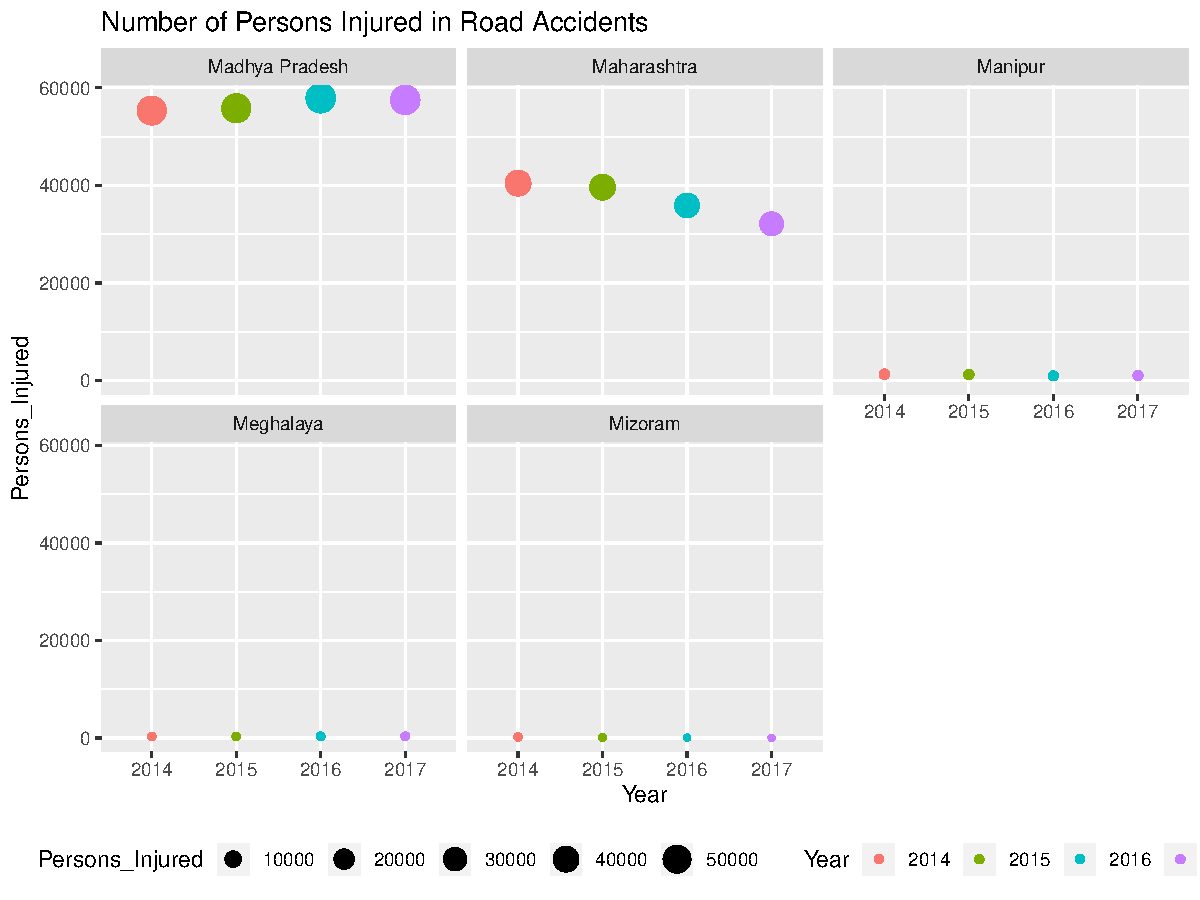
\includegraphics{TutorialNotebook_files/figure-latex/unnamed-chunk-21-1.pdf}
\caption{A simple graphic produced with \textbf{ggplot2}}
\end{figure}

The beauty of \textbf{ggplot2} package lies in adding of layers. Thus we
can plot ggplot object(namely \texttt{p1}) directl, or add more layers
like \texttt{title}, \texttt{theme} of graph. Thus, we see the ease of
use that \textbf{ggplot2} package provides.

We are now in position to plot spatial objects using \textbf{gmap}
package, which is based on \textbf{ggplot2} package.

\hypertarget{ggmap}{%
\subsection{ggmap}\label{ggmap}}

In the following steps we will create a map to show the total number of
persons injured in road accidents in India(instead of few selected
states). This will require the usage of \textbf{ggmap} package, which is
based on the \textbf{ggplot2} package. Like \textbf{ggplot2},
\textbf{ggmap} package also requires requires data (including spatial
data) to be supplied as \texttt{data.frame}. We use \texttt{tidy()}
method from package \texttt{broom} to coerce spatial object to a data
frame object. The generic plot() functions then, can use
\texttt{Spatial*} objects directly.

\begin{Shaded}
\begin{Highlighting}[]
\NormalTok{states_df <-}\StringTok{ }\NormalTok{broom}\OperatorTok{::}\KeywordTok{tidy}\NormalTok{(states)}
\end{Highlighting}
\end{Shaded}

\begin{verbatim}
## Regions defined for each Polygons
\end{verbatim}

\textbf{Note} : The \texttt{tidy()} method coerces the spatial data
object into a data frame. In this process of coercing, we lost the
attribute information of states object. We add it back using the
\texttt{left\_join} function from* \textbf{dplyr} package.

\begin{Shaded}
\begin{Highlighting}[]
\KeywordTok{library}\NormalTok{(dplyr)}
\CommentTok{# head(states_df, n = 2) # Investigate the tide-ied data}
\NormalTok{states}\OperatorTok{$}\NormalTok{id <-}\StringTok{ }\KeywordTok{row.names}\NormalTok{(states) }\CommentTok{#Allocate an id variable to sp data}
\CommentTok{# head(states@data, n = 2) # A check before we join}
\NormalTok{states_df <-}\StringTok{ }\KeywordTok{left_join}\NormalTok{(states_df, states}\OperatorTok{@}\NormalTok{data)}
\end{Highlighting}
\end{Shaded}

\begin{verbatim}
## Joining, by = "id"
\end{verbatim}

Now our \texttt{states\_df} object contains geospatial cooridnates
information alongside the attribute information of road accidents in
India. It is now straightforward to produce a map with \textbf{ggplot2}.

\begin{Shaded}
\begin{Highlighting}[]
\NormalTok{map <-}\StringTok{ }\KeywordTok{ggplot}\NormalTok{(}\DataTypeTok{data =}\NormalTok{ states_df, }\KeywordTok{aes}\NormalTok{(}\DataTypeTok{x =}\NormalTok{ long, }\DataTypeTok{y =}\NormalTok{ lat, }\DataTypeTok{group =}\NormalTok{ group, }\DataTypeTok{fill =}\NormalTok{ State.UT.wise.Total.Number.of.Persons.Injured.in.Road.Accidents.during...}\DecValTok{2015}\NormalTok{))}\OperatorTok{+}\StringTok{ }\CommentTok{# define variables}
\StringTok{  }\KeywordTok{geom_polygon}\NormalTok{() }\OperatorTok{+}\StringTok{ }\CommentTok{# Plot the states}
\StringTok{  }\KeywordTok{coord_equal}\NormalTok{() }\OperatorTok{+}\StringTok{ }\CommentTok{# fixed x & y scales}
\StringTok{  }\KeywordTok{labs}\NormalTok{(}\DataTypeTok{x =} \StringTok{"longitude"}\NormalTok{, }\DataTypeTok{y =} \StringTok{"latitude"}\NormalTok{, }\DataTypeTok{fill =} \StringTok{"Number of Persons_Injured"}\NormalTok{) }\OperatorTok{+}\StringTok{ }\CommentTok{#Labels}
\StringTok{  }\KeywordTok{ggtitle}\NormalTok{(}\StringTok{"Road Accidents in India (2015)"}\NormalTok{) }\OperatorTok{+}\StringTok{ }\CommentTok{#title}
\StringTok{  }\KeywordTok{scale_fill_gradient}\NormalTok{(}\DataTypeTok{low =} \StringTok{"white"}\NormalTok{, }\DataTypeTok{high =} \StringTok{"green"}\NormalTok{) }\CommentTok{#colours}
\NormalTok{map }\CommentTok{#Figure 4 }
\end{Highlighting}
\end{Shaded}

\begin{figure}
\centering
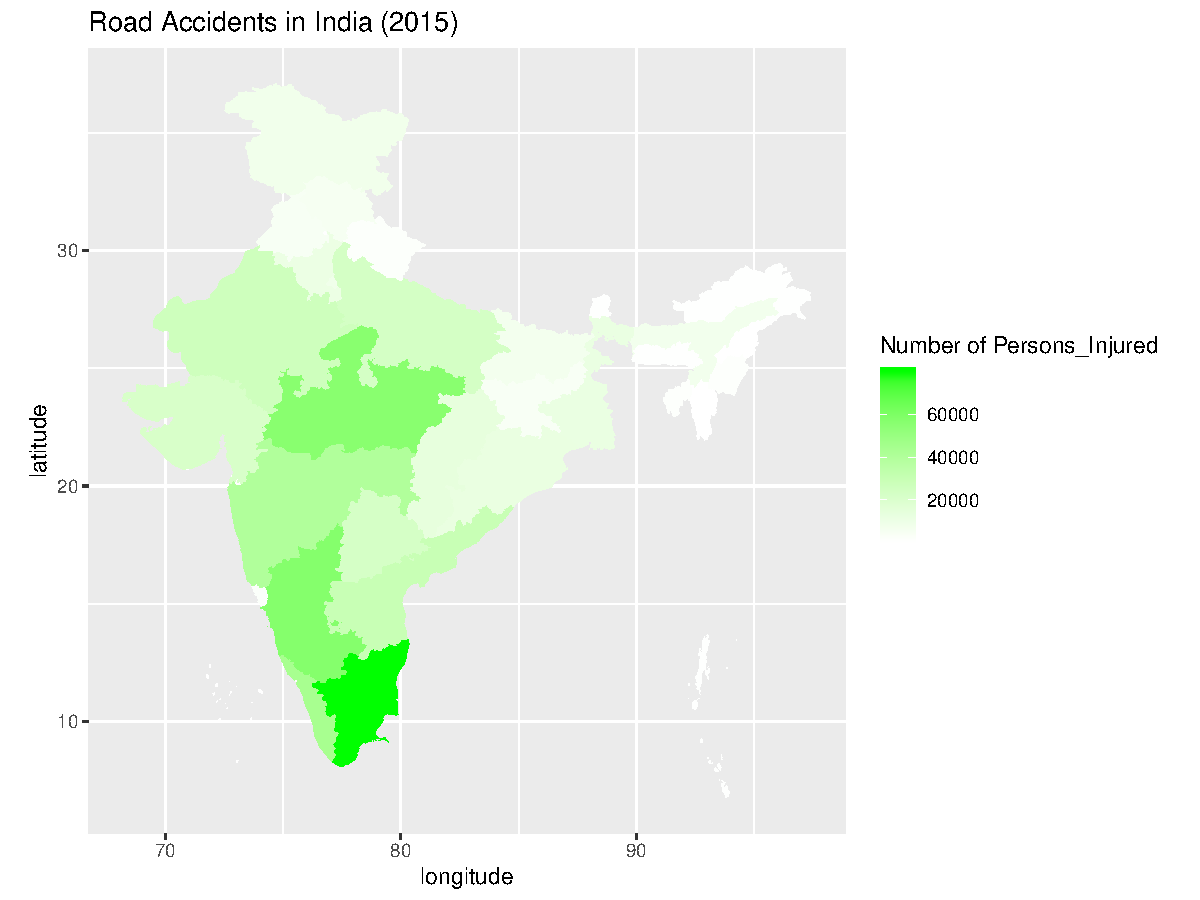
\includegraphics{TutorialNotebook_files/figure-latex/unnamed-chunk-24-1.pdf}
\caption{Map of Number of persons injured due to Road Accidents in
India}
\end{figure}

We can add more description from other packages. As an example, you can
add a direction symbol using ``ggsn'' package as following

\begin{Shaded}
\begin{Highlighting}[]
\NormalTok{map }\OperatorTok{+}\StringTok{ }\NormalTok{ggsn}\OperatorTok{::}\KeywordTok{blank}\NormalTok{() }\OperatorTok{+}\StringTok{ }\NormalTok{ggsn}\OperatorTok{::}\KeywordTok{north}\NormalTok{(states_df) }\CommentTok{#Output not shown.}
\end{Highlighting}
\end{Shaded}

\clearpage

\hypertarget{analysing-spatial-data}{%
\section{5. Analysing Spatial Data}\label{analysing-spatial-data}}

In the previous sections, we have learnt the nuts and bolts of spatial
data analysis. Its now time to create put things together and create a
bigger picture, conveying more information. So far we have drawn plots
and graphs with limited information to display. In the \textbf{ggplot2}
example, we drew the comaprisons of number of persons injured in road
accidents among few states. The infograph was incapable to plot such a
graph for every state, due to plotting space constraint. Hence we were
restricted to fewer states to avoid clutter. Later on we draw the map to
represent information for all the states, but for a single year.

We are now in position to do some analysis, leveraging the power of
spatial data. We make use of faceting for maps, and draw comparisons
over the years for all states - side by side. As a first step - we need
to prepare the data for faceting. Remember we saved our \texttt{df.m}
object in section 4. Its time now to fetch it back.

\begin{Shaded}
\begin{Highlighting}[]
\CommentTok{# load the saved R object}
\NormalTok{accidents_df<-}\StringTok{ }\KeywordTok{readRDS}\NormalTok{(}\DataTypeTok{file =} \StringTok{"Data/Statewise_Yearly_Road_Accidents_India.Rds"}\NormalTok{) }
\end{Highlighting}
\end{Shaded}

Next we prepare our data for plotting. This involves converting the
spatial object into a data frame object, and join it with non-spatial
data frame containg more attributes. Do not forget to manually correct
the typographical errors.

\begin{Shaded}
\begin{Highlighting}[]
\CommentTok{# Creating a data frame for plotting}
\NormalTok{states <-}\StringTok{  }\NormalTok{states_raw}

\NormalTok{states_df <-}\StringTok{ }\NormalTok{broom}\OperatorTok{::}\KeywordTok{tidy}\NormalTok{(states)}
\KeywordTok{head}\NormalTok{(states_df)}
\end{Highlighting}
\end{Shaded}

\begin{verbatim}
## # A tibble: 6 x 7
##    long   lat order hole  piece group id   
##   <dbl> <dbl> <int> <lgl> <chr> <chr> <chr>
## 1  92.9  12.9     1 FALSE 1     0.1   0    
## 2  92.9  12.9     2 FALSE 1     0.1   0    
## 3  92.9  12.9     3 FALSE 1     0.1   0    
## 4  92.9  12.9     4 FALSE 1     0.1   0    
## 5  92.9  12.9     5 FALSE 1     0.1   0    
## 6  92.9  12.9     6 FALSE 1     0.1   0
\end{verbatim}

\begin{Shaded}
\begin{Highlighting}[]
\NormalTok{states}\OperatorTok{@}\NormalTok{data <-}\StringTok{ }\KeywordTok{edit}\NormalTok{(states}\OperatorTok{@}\NormalTok{data)}
\NormalTok{states}\OperatorTok{$}\NormalTok{id <-}\StringTok{  }\KeywordTok{row.names}\NormalTok{(states)}
\KeywordTok{head}\NormalTok{(states}\OperatorTok{@}\NormalTok{data)}
\end{Highlighting}
\end{Shaded}

\begin{verbatim}
##                       ST_NM id
## 0 Andaman & Nicobar Islands  0
## 1         Arunachal Pradesh  1
## 2                     Assam  2
## 3                     Bihar  3
## 4                Chandigarh  4
## 5              Chhattisgarh  5
\end{verbatim}

\begin{Shaded}
\begin{Highlighting}[]
\NormalTok{states_df <-}\StringTok{ }\KeywordTok{left_join}\NormalTok{(states_df, states}\OperatorTok{@}\NormalTok{data)}
\KeywordTok{head}\NormalTok{(states_df)}
\end{Highlighting}
\end{Shaded}

\begin{verbatim}
## # A tibble: 6 x 8
##    long   lat order hole  piece group id    ST_NM                    
##   <dbl> <dbl> <int> <lgl> <chr> <chr> <chr> <chr>                    
## 1  92.9  12.9     1 FALSE 1     0.1   0     Andaman & Nicobar Islands
## 2  92.9  12.9     2 FALSE 1     0.1   0     Andaman & Nicobar Islands
## 3  92.9  12.9     3 FALSE 1     0.1   0     Andaman & Nicobar Islands
## 4  92.9  12.9     4 FALSE 1     0.1   0     Andaman & Nicobar Islands
## 5  92.9  12.9     5 FALSE 1     0.1   0     Andaman & Nicobar Islands
## 6  92.9  12.9     6 FALSE 1     0.1   0     Andaman & Nicobar Islands
\end{verbatim}

\begin{Shaded}
\begin{Highlighting}[]
\CommentTok{# Preparing the Spatial Object}
\NormalTok{states_df <-}\StringTok{ }\KeywordTok{left_join}\NormalTok{(states_df, accidents_df)}
\end{Highlighting}
\end{Shaded}

We now plot the data and see the results.

\begin{Shaded}
\begin{Highlighting}[]
\KeywordTok{ggplot}\NormalTok{(}\DataTypeTok{data =}\NormalTok{ states_df,}
       \KeywordTok{aes}\NormalTok{(}\DataTypeTok{x =}\NormalTok{ long, }\DataTypeTok{y =}\NormalTok{ lat, }\DataTypeTok{fill =}\NormalTok{ Persons_Injured, }\DataTypeTok{group =}\NormalTok{ group)) }\OperatorTok{+}\StringTok{ }\CommentTok{#defining Variables}
\StringTok{  }\KeywordTok{geom_polygon}\NormalTok{() }\OperatorTok{+}\StringTok{ }\CommentTok{#plot states map}
\StringTok{  }\KeywordTok{geom_path}\NormalTok{(}\DataTypeTok{colour =} \StringTok{"black"}\NormalTok{, }\DataTypeTok{lwd =} \FloatTok{0.05}\NormalTok{) }\OperatorTok{+}\StringTok{ }\CommentTok{# states borders}
\StringTok{  }\KeywordTok{coord_equal}\NormalTok{() }\OperatorTok{+}\StringTok{ }\CommentTok{#fixed x and y scales}
\StringTok{  }\KeywordTok{facet_wrap}\NormalTok{(}\OperatorTok{~}\StringTok{ }\NormalTok{Year) }\OperatorTok{+}\StringTok{ }\CommentTok{# one plot per year}
\StringTok{  }\KeywordTok{scale_fill_gradient}\NormalTok{(}\DataTypeTok{low =} \StringTok{"white"}\NormalTok{, }\DataTypeTok{high =} \StringTok{"green"}\NormalTok{,}
                      \DataTypeTok{name =} \StringTok{"No. of Persons Injured"}\NormalTok{) }\OperatorTok{+}\StringTok{ }\CommentTok{# legend options}
\StringTok{  }\KeywordTok{theme}\NormalTok{(}\DataTypeTok{axis.text =} \KeywordTok{element_blank}\NormalTok{(), }\CommentTok{# remove axis lables}
        \DataTypeTok{axis.title =} \KeywordTok{element_blank}\NormalTok{(), }\CommentTok{# remove axis titles}
        \DataTypeTok{axis.ticks =} \KeywordTok{element_blank}\NormalTok{()) }\CommentTok{# remove axis ticks}
\end{Highlighting}
\end{Shaded}

\begin{figure}
\centering
\includegraphics{TutorialNotebook_files/figure-latex/unnamed-chunk-28-1.pdf}
\caption{Figure depicting the number of persons injured in India due to
road accidents over the years}
\end{figure}

\clearpage

\hypertarget{references}{%
\section{References}\label{references}}

Lovelace, R., Cheshire, J. and Oldroyd, R. (2017). Introduction to
visualising spatial data in R. {[}ebook{]} Available at:
\url{https://github.com/Robinlovelace/Creating-maps-in-R} {[}Accessed 18
May 2017{]}.

Sadler, J. (2019). Introduction to GIS with R. {[}online{]} Jesse
Sadler. Available at:
\url{https://www.jessesadler.com/post/gis-with-r-intro/} {[}Accessed 25
Dec.~2019{]}.

Brunsdon, C. and Comber, L. (2015). An Introduction to R for Spatial
Analysis and Mapping. 1st ed.


\end{document}
